\section{Introducción}
\subsection{Contexto General}

Una imagen vale 1000 palabras. Esa es una frase que muchos hemos escuchado en algún momento de nuestras vidas, y que probablemente ya sepamos qué significa con sólo leerla. Tener la capacidad de otorgar una explicación a través de visualizar la información hace que las ideas sean mucho más fáciles de comunicar a otros. Cuando tenemos la capacidad de visualizar la información, no sólo se facilita la tarea de explicar, si no también la de aprender.

Por ejemplo, si tenemos un gráfico de series de tiempo, típicamente pondremos el rango de tiempo en el eje X, así como un valor cambiante en el eje Y que puede representar una temperatura, uso de CPU, precios de acciones, visitas a un sitio web, etc. Este setup nos permite identificar cómo cambia esta variable durante el tiempo, así como identificar patrones, tendencias, cambios súbitos y mucho más. Graficar es una excelente herramienta para el estudio de este tipo de información, dándonos una clara estructura para la intepretación de su comportamiento en el paso del tiempo, facilitando la comparación de distintos momentos y otorgarle un significado a los mismos. 

Todo esto es posible gracias a la \textbf{visualización}, que podemos entender como el uso de representaciones visuales interactivas, asistidas por computadora, para ayudar a la cognición.~\cite{card1999readings}.

A pesar de esta definición, que posiciona la visualización como una herramienta que sienta sus bases en la computación y la tecnología de nuestra era, sus orígenes se remontan a la antigüedad. Las civilizaciones tempranas utilizaron distintos métodos para representar datos de forma visual, como el mapa estelar de Suzhou de la dinastía Song en China, creado en 1193, que mostraba 1.434 estrellas agrupadas en 280 constelaciones. Este y otros ejemplos históricos nos demuestran el deseo humano de centrar sus esfuerzos en simplificar información compleja en formas comprensibles y accesibles, utilizando representaciones visuales que potencian nuestra capacidad para observar patrones, relaciones y significados que de otro modo pasarían desapercibidos.

Sin embargo, en la era contemporánea, la llegada de los computadores y el software ha revolucionado nuestra capacidad de manejar la información. Es gracias a estos avances tecnológicos que podemos procesar grandes volúmenes de información compleja, que normalmente no podríamos haber procesado sin la aparición de software específico para este objetivo. Nos referiremos a este tipo de datos como \textbf{Macrodatos} o \textbf{Big Data}\cite{mcafee2012bigdata}.

\subsubsection{Big Data}

La definición de \textit{Big Data} corresponde a la información de gran volúmen, gran velocidad y gran variedad que requiere formas innovadoras y eficientes para su procesamiento. Sin embargo, este término se popularizó al rededor del año 2012~\cite{diebold2012bigdata}, y lo que se consideraba \textit{Big Data} en el pasado es de mucha menor magnitud de lo que se considera hoy en día. Así mismo, la magnitud de estos datos en un futuro será mayor, ya que las capacidades de almacenamiento y procesamiento aumentarán.

Por tanto, se considerarán algunas características esenciales para asegurarnos de que estamos lidiando con macrodatos.
\begin{enumerate}
    \item \textbf{Variedad}: \\
        El conjunto de datos es heterogéneo, y normalmente no posee una estructura concreta para su procesamiento de manera nativa.
    \item \textbf{Velocidad}: \\
        Se refiera a la rapidez con la que los datos se generan. Normalmente los tipos de datos a analizar están en tiempo real, y generan nuevos datos a una frecuencia alta.
    \item \textbf{Volumen}: \\
        La cantidad de datos es significativa para el sistema donde se está trabajando y la tecnología actual.
\end{enumerate}

Otra característica importante a considerar de esta definición, es que estos datos son \textbf{inútiles} por sí solos~\cite{gandomi2015beyond}. La relevancia de este gran volúmen de información proviene del conjunto de los datos y la interpretación de los mismos. 

Manejar \textit{Macrodatos} es una tarea que ha sido simplificada con la ayuda de software como \textit{Tableu}, \textit{Power BI} o \textit{D3.js}. Estas herramientas otorgan al usuario caracterísiticas como hacer zoom, filtrar e incluso actualizaciones en vivo de las series de tiempo que se estudian. Así mismo, podemos encontrar bibliotecas de \textit{Python} que entregan estas mismas características a los desarrolladores, tales como \textit{Plotly} o \textit{Bokeh}. El uso de la visualización para analizar macrodatos posee los mismos beneficios que se han mencionado con anterioridad, lo cual es relevante ya que podría mejorar la toma de decisiones sobre los mismos en un $77\%$~\cite{ali2016bigdata}.

Al graficar una serie de datos, típicamente debemos recorrer cada punto contenido en el vector, generando una complejidad temporal $O(n)$. Este crecimiento lineal implica que, a mayor cantidad de datos, más tiempo requeriremos para graficarlos de manera proporcional. Por ejemplo, en la figura \ref{add_trace_plotly} se muestra cómo graficar una serie con aproximadamente 350 mil puntos toma alrededor de 1.5 segundos, un tiempo considerable al considerar que estas visualizaciones deben ser ágiles para realizar análisis o investigaciones en tiempo real.

Además del rendimiento, cuando trabajamos con series temporales extremadamente densas o con puntos altamente consecutivos entre sí, obtenemos gráficos difíciles de interpretar visualmente. Este problema genera la impresión de gráficos comprimidos o saturados ("squashed"), dificultando enormemente su análisis, como puede observarse claramente en la Figura \ref{squashed_plot}, que representa la lectura de un sensor colocado en un puente.

El creciente volumen de datos en contextos de Big Data nos obliga a repensar los fundamentos mismos de la visualización. Si graficar cientos de miles de puntos ya representa un reto técnico y cognitivo, ¿qué ocurre cuando nos enfrentamos a millones o incluso miles de millones de registros? En estos casos, la visualización deja de ser una simple representación directa de los datos y se transforma en un proceso de síntesis y decisión: ¿qué se debe mostrar, qué se puede omitir, y cómo evitar distorsionar la información en el camino?

\subsubsection{Downsampling}

Mejorar la eficiencia de los procesos que permiten la visualización es una manera de reducir los tiempos de cómputo, sin embargo esto no es suficiente por sí solo. Aún con estas mejoras, llega una cantidad de puntos que simplemente no es viable visualizar en tiempo real. Así mismo, la legibilidad de los gráficos no se resuelve con estos avances.

Es complejo escapar de esta problemática, ya que no podemos reducir la complejidad temporal lineal a menos que \textbf{no grafiquemos todos los puntos}.

Bajo esa idea surge la técnica conocida como \textit{downsampling}, la cual consiste en seleccionar solo un subconjunto de los puntos originales para ser graficados. A diferencia de métodos que generan nuevos datos mediante agregaciones o promedios, el \textit{downsampling} busca preservar puntos existentes del conjunto original que sean representativos de su comportamiento general. Su objetivo no es reemplazar el análisis detallado, sino facilitar la interpretación visual de grandes volúmenes de datos en contextos donde mostrar todos los puntos no es viable ni útil~\cite{steinarsson2013downsampling}. Esta técnica permite reducir el tiempo de renderizado y evitar la saturación visual sin comprometer, en teoría, la percepción de patrones relevantes. No obstante, su aplicación exige un criterio claro: ¿qué puntos se deben conservar para que la visualización siga siendo fiel a los datos?

Una solución común al problema del exceso de puntos en las series de tiempo es el uso de técnicas de downsampling, las cuales seleccionan un subconjunto representativo de los datos originales para graficar. Esto permite mejorar el rendimiento y la legibilidad sin comprometer significativamente la percepción de patrones relevantes. Existen múltiples algoritmos diseñados con este fin, los cuales serán analizados en detalle en la sección de Evaluación de Alternativas\ref{alternatives}.

El grupo de investigación \textbf{PreDiCT.IDLab}, afiliado a la Universidad de Gante en Bélgica, ha desarrollado e investigado activamente métodos avanzados para la visualización eficiente de series de tiempo. Entre sus contribuciones destaca la herramienta tsdownsample, un conjunto de algoritmos de alto rendimiento diseñados específicamente para realizar downsampling en contextos de visualización~\cite{tsdownsample}, la cual implementa los algoritmos ya mencionados para ser utilizados en \textit{python}.

Otra biblioteca de gran utilidad creada por estos académicos es \textit{plotly-resampler}~\cite{plotly-resampler}, la cual integra este procesamiento de manera directa en \textit{plotly}. A pesar de el preprocesamiento necesario para generar una submuestra de una serie de tiempo, aún así podemos ver diferencias significativas en el tiempo necesario para la visualización de conjuntos grandes de información.

Esta mejora es evidente en la Figura \ref{plotly_vs_resampler}, donde podemos visualizar cómo al usar \textit{plotly-resampler} al añadir una línea en el gráfico reduce el tiempo de ejecución significativamente, a pesar de que llama a la función original de \textit{plotly} y procesa el vector original.

En definitiva, usar estrategias de \textit{downsample} es una opción muy útil a la hora de visualizar una serie de tiempo con muchos puntos, ya que permite mejorar la legibilidad, tiempo de renderización y, a causa de esto, la cognición de los datos que se están estudiando.
% to do: hacer una figura que compare plotly y plotly resampler para decir miren asi evolucionan las curvas, y explicar por qué

\subsection{Presentación del Problema}

A pesar de todas las ventajas que ofrece el uso de técnicas de \textit{downsampling} —como la mejora en el tiempo de renderizado, la reducción de la sobrecarga cognitiva y una experiencia más fluida al visualizar datos densos—, estas no necesariamente abordan todos los aspectos posibles de optimización dentro del proceso de visualización de series de tiempo.

Por ejemplo, herramientas como \textit{tsdownsample} permiten reducir la cantidad de puntos a representar, generando así gráficos más livianos y veloces. Sin embargo, incluso los datos ya reducidos siguen representándose con estructuras estándar que pueden ocupar un espacio considerable en memoria. En otras palabras, se reduce la cantidad de información a procesar, pero no necesariamente el tamaño de esa información en términos de espacio ocupado.

Esto plantea una nueva dimensión del problema: si ya hemos logrado disminuir significativamente el tiempo requerido para visualizar datos, ¿por qué no aprovechar esa mejora para optimizar también el espacio que ocupan los datos resultantes? Es decir, en lugar de mantenernos solo en la reducción de puntos, podríamos buscar formas de representar esa información de manera más eficiente, reduciendo aún más el tamaño total ocupado sin perder la capacidad de analizarla visualmente.

Esta inquietud da paso a explorar otras técnicas que permitan una representación más compacta de los datos, y que puedan integrarse con las estrategias de \textit{downsampling} existentes para alcanzar un nuevo nivel de eficiencia.


\begin{figure}
    \centering
    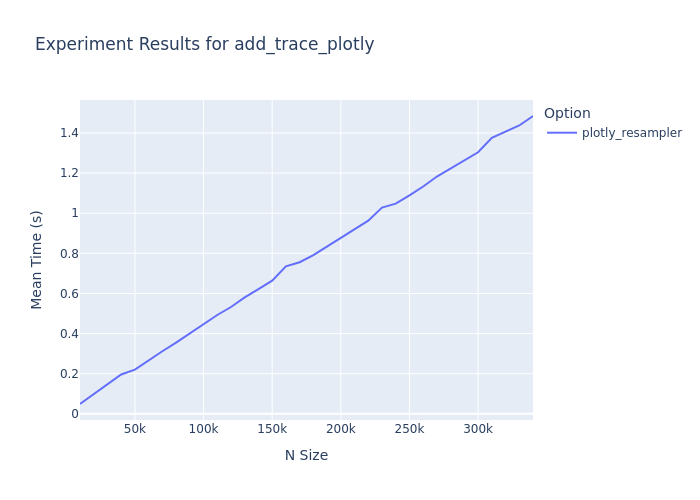
\includegraphics[width=0.9\linewidth]{introduction/images/add_trace_plotly.png}
    \title{figure}
    \caption{Tiempo promedio en segundos de graficar N cantidad de puntos usando la librería plotly.}
    \label{add_trace_plotly}
\end{figure}

\begin{figure}
    \centering
    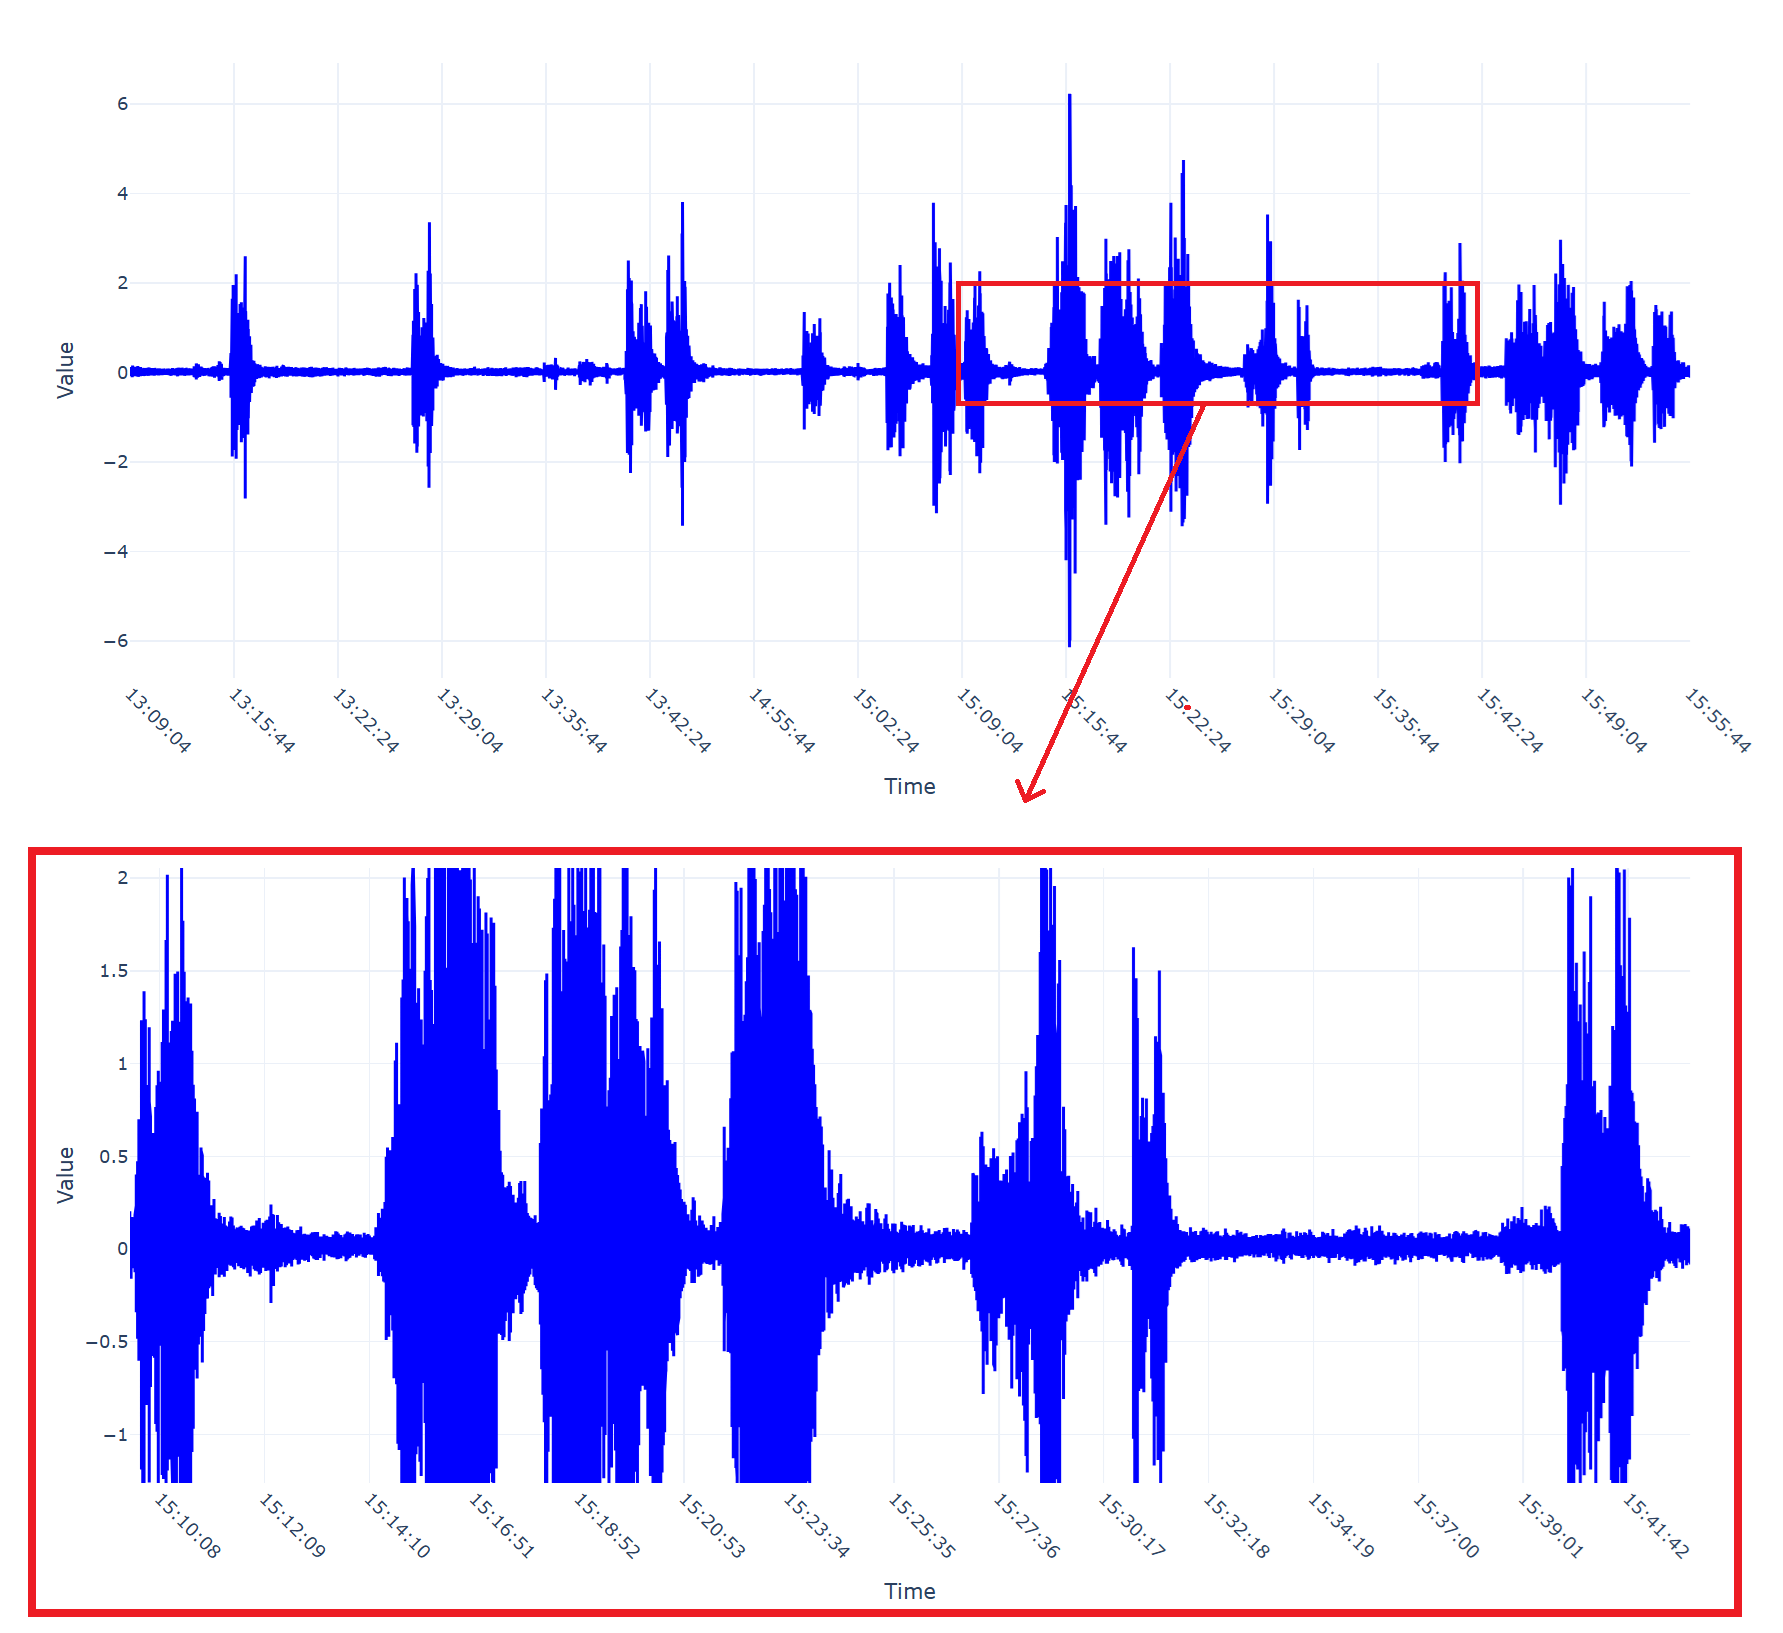
\includegraphics[width=0.9\linewidth]{introduction/images/squashed_plot.png}
    \caption{Serie de tiempo con aproximadamante 350,000 puntos con valores del sensor de un puente. Al ser demasiados puntos por segundo, es difícil identificar el comportamiento del sensor en cada segundo.}
    \label{squashed_plot}
\end{figure}

\begin{figure}
    \centering
    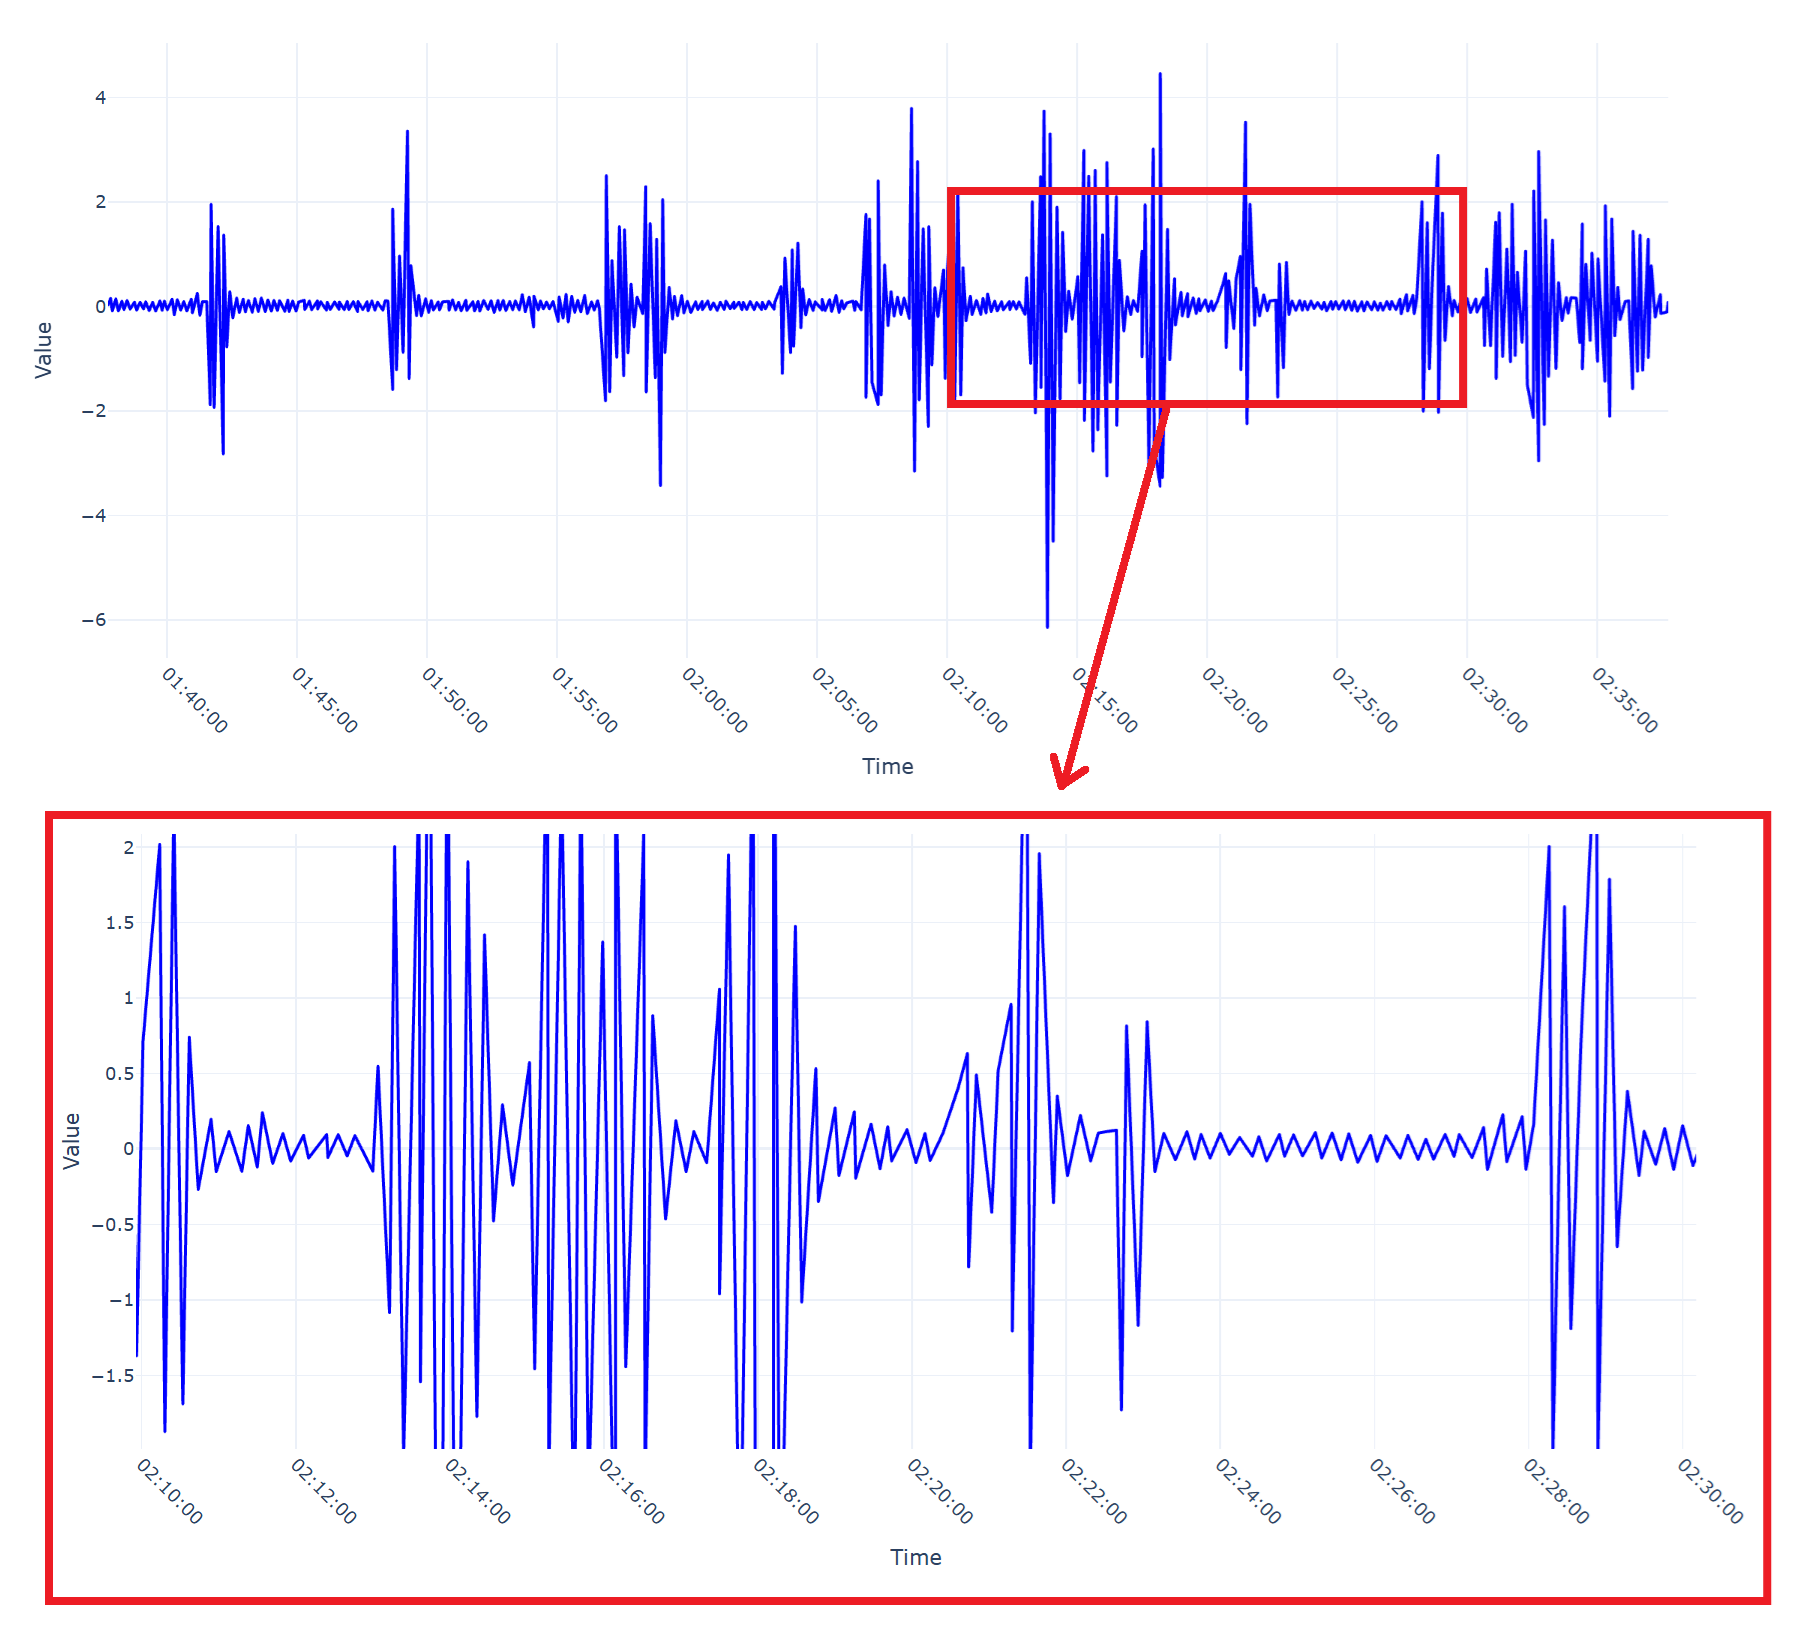
\includegraphics[width=0.9\linewidth]{introduction/images/downsample.png}
    \caption{Downsample de erie de tiempo con aproximadamante 350,000 puntos con valores del sensor de un puente.}
    \label{downsample}
\end{figure}

\begin{figure}
    \centering
    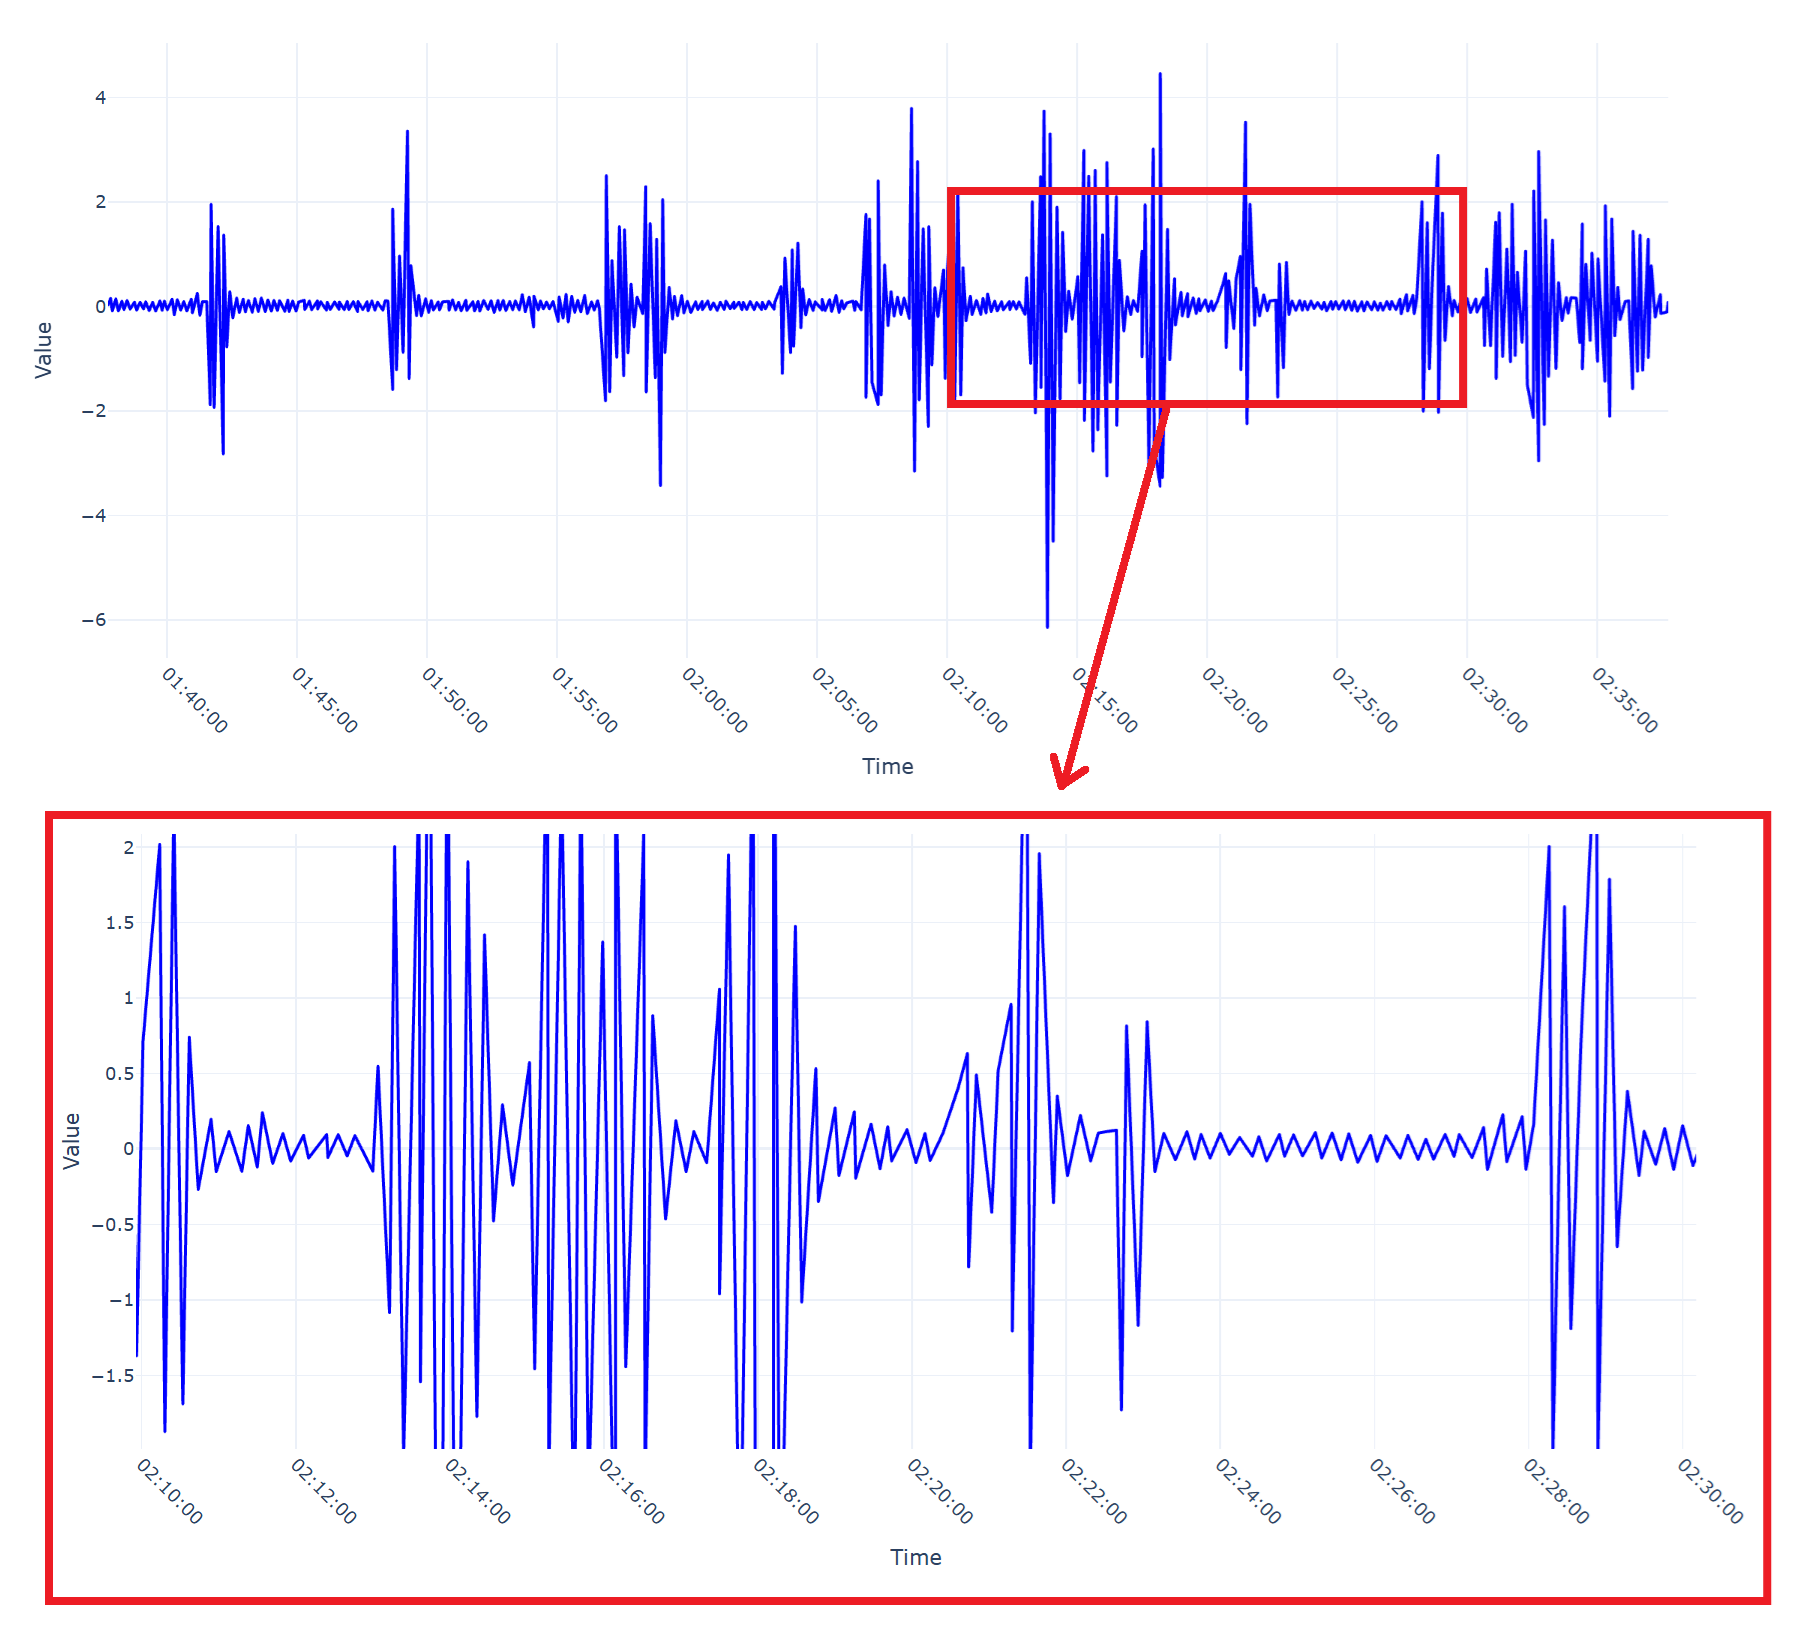
\includegraphics[width=0.9\linewidth]{introduction/images/downsample.png}
    \caption{Downsample de erie de tiempo con aproximadamante 350,000 puntos con valores del sensor de un puente.}
    \label{plotly_vs_resampler}
\end{figure}